\documentclass{standalone}

\usepackage{tikz}
\usepackage{pgfplots}
\usetikzlibrary{calc}
\pgfplotsset{compat=1.15}

\begin{document}

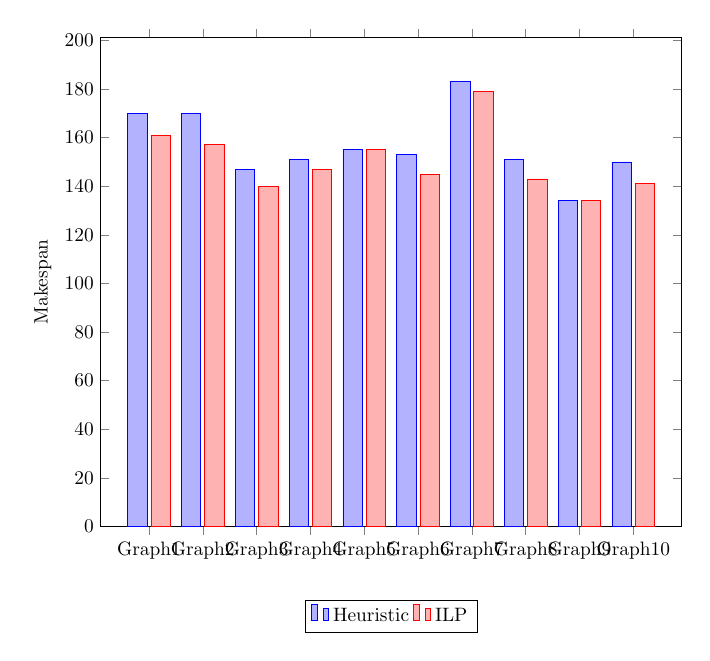
\begin{tikzpicture}[scale=0.7]
    \begin{axis}[
        width=\textwidth,
       % x tick label style={/pgf/number format/1000 sep=},
				symbolic x  coords={Graph1,Graph2,Graph3,Graph4, Graph5,Graph6,Graph7,Graph8,Graph9,Graph10},
        ylabel=Makespan,
				ymin=0,
        %enlargelimits=0.15,
        legend style={at={(0.5,-0.15)},
        anchor=north,legend columns=-1},
        ybar,
        bar width=10pt,
        ]
        \addplot
        coordinates {
				  (Graph1,170)
(Graph2,170)
(Graph3,147)
(Graph4,151)
(Graph5,155)
(Graph6,153)
(Graph7,183)
(Graph8,151)
(Graph9,134)
(Graph10,150)
				};
        \addplot
        coordinates {
				  (Graph1,161)
(Graph2,157)
(Graph3,140)
(Graph4,147)
(Graph5,155)
(Graph6,145)
(Graph7,179)
(Graph8,143)
(Graph9,134)
(Graph10,141)
				};
        
        \legend{Heuristic,ILP}
    \end{axis}
\end{tikzpicture}

\end{document}